\documentclass[dissertation.tex]{subfiles} 
\begin{document}

\chapter{The Large Hadron Collider}
\label{chap:The Large Hadron Collider}

At a 2010-2011 energy of 3.5 TeV/beam (7 TeV/beam design \cite{LHC_paper}) and maximum instantaneous luminosity of $3.55 \times 10^{33}\mbox{ cm}^{-2}\mbox{ s}^{-1}$ \cite{CMS_2011_summary} ($10^{34}\mbox{ cm}^{-2}\mbox{ s}^{-1}$ design \cite{LHC_paper}), the Large Hadron Collider (LHC) is the highest energy and highest intensity proton-proton collider ever built.  Its purpose is to allow the four LHC experiments to explore TeV scale physics.  For CMS and ATLAS, this implies examining the origins of EWSB via searches for the SM Higgs boson and physical phenomena not predicted by the SM that may explain the mass hierarchy in the SM.  It also includes searches for possible dark matter candidates that are often proposed to have masses at the weak scale.  The LHC needs to provide high energy proton collisions because the masses of the sought-after particles are higher than those already incorporated into the SM.  It must also provide an unprecedented collision rate because signatures of the Higgs boson and physics beyond the SM are very rare compared to SM processes.

The rest of this chapter is devoted to an overview of the LHC machine.  Section~\ref{sec:Design Considerations and Performance Limitations} gives the overall layout of the machine and design choices made in light of energy and luminosity demands.  Section~\ref{sec:Beam Injection} describes the LHC injection scheme.  The different types of magnets and their functions is illustrated in Section~\ref{sec:Magnets and Cryogenics}, and finally the radiofrequency cavities are covered in Section~\ref{sec:Radiofrequency Cavities}.  Unless otherwise noted, all information in this chapter comes from ref. \cite{LHC_paper}.

\section{Design Considerations and Performance Limitations}
\label{sec:Design Considerations and Performance Limitations}

The layout of the 26.7-km long \cite{LHC_public} LHC ring, located $\sim100$ m underground on the border between France and Switzerland northwest of Geneva, is shown in Figure~\ref{fig:LHC_layout}.  The two circulating beams of protons travel in opposite directions, colliding only at the experimental points.  There are eight straight sections, each $\sim528$ m long, and eight arcs, each made of 23 106.9-m long arc cells.  Beam crossings occur in four of the straight sections.  The arcs contain six 14.3-m long dipole magnets, the cryogenics to cool the magnets, and short straight sections (SSS) with focusing and corrector magnets.  The high luminosity experiments CMS and ATLAS are located diametrically opposite each other on the ring, ensuring that in principle each should receive the same integrated luminosity from the LHC.

\begin{figure}
	\centering
	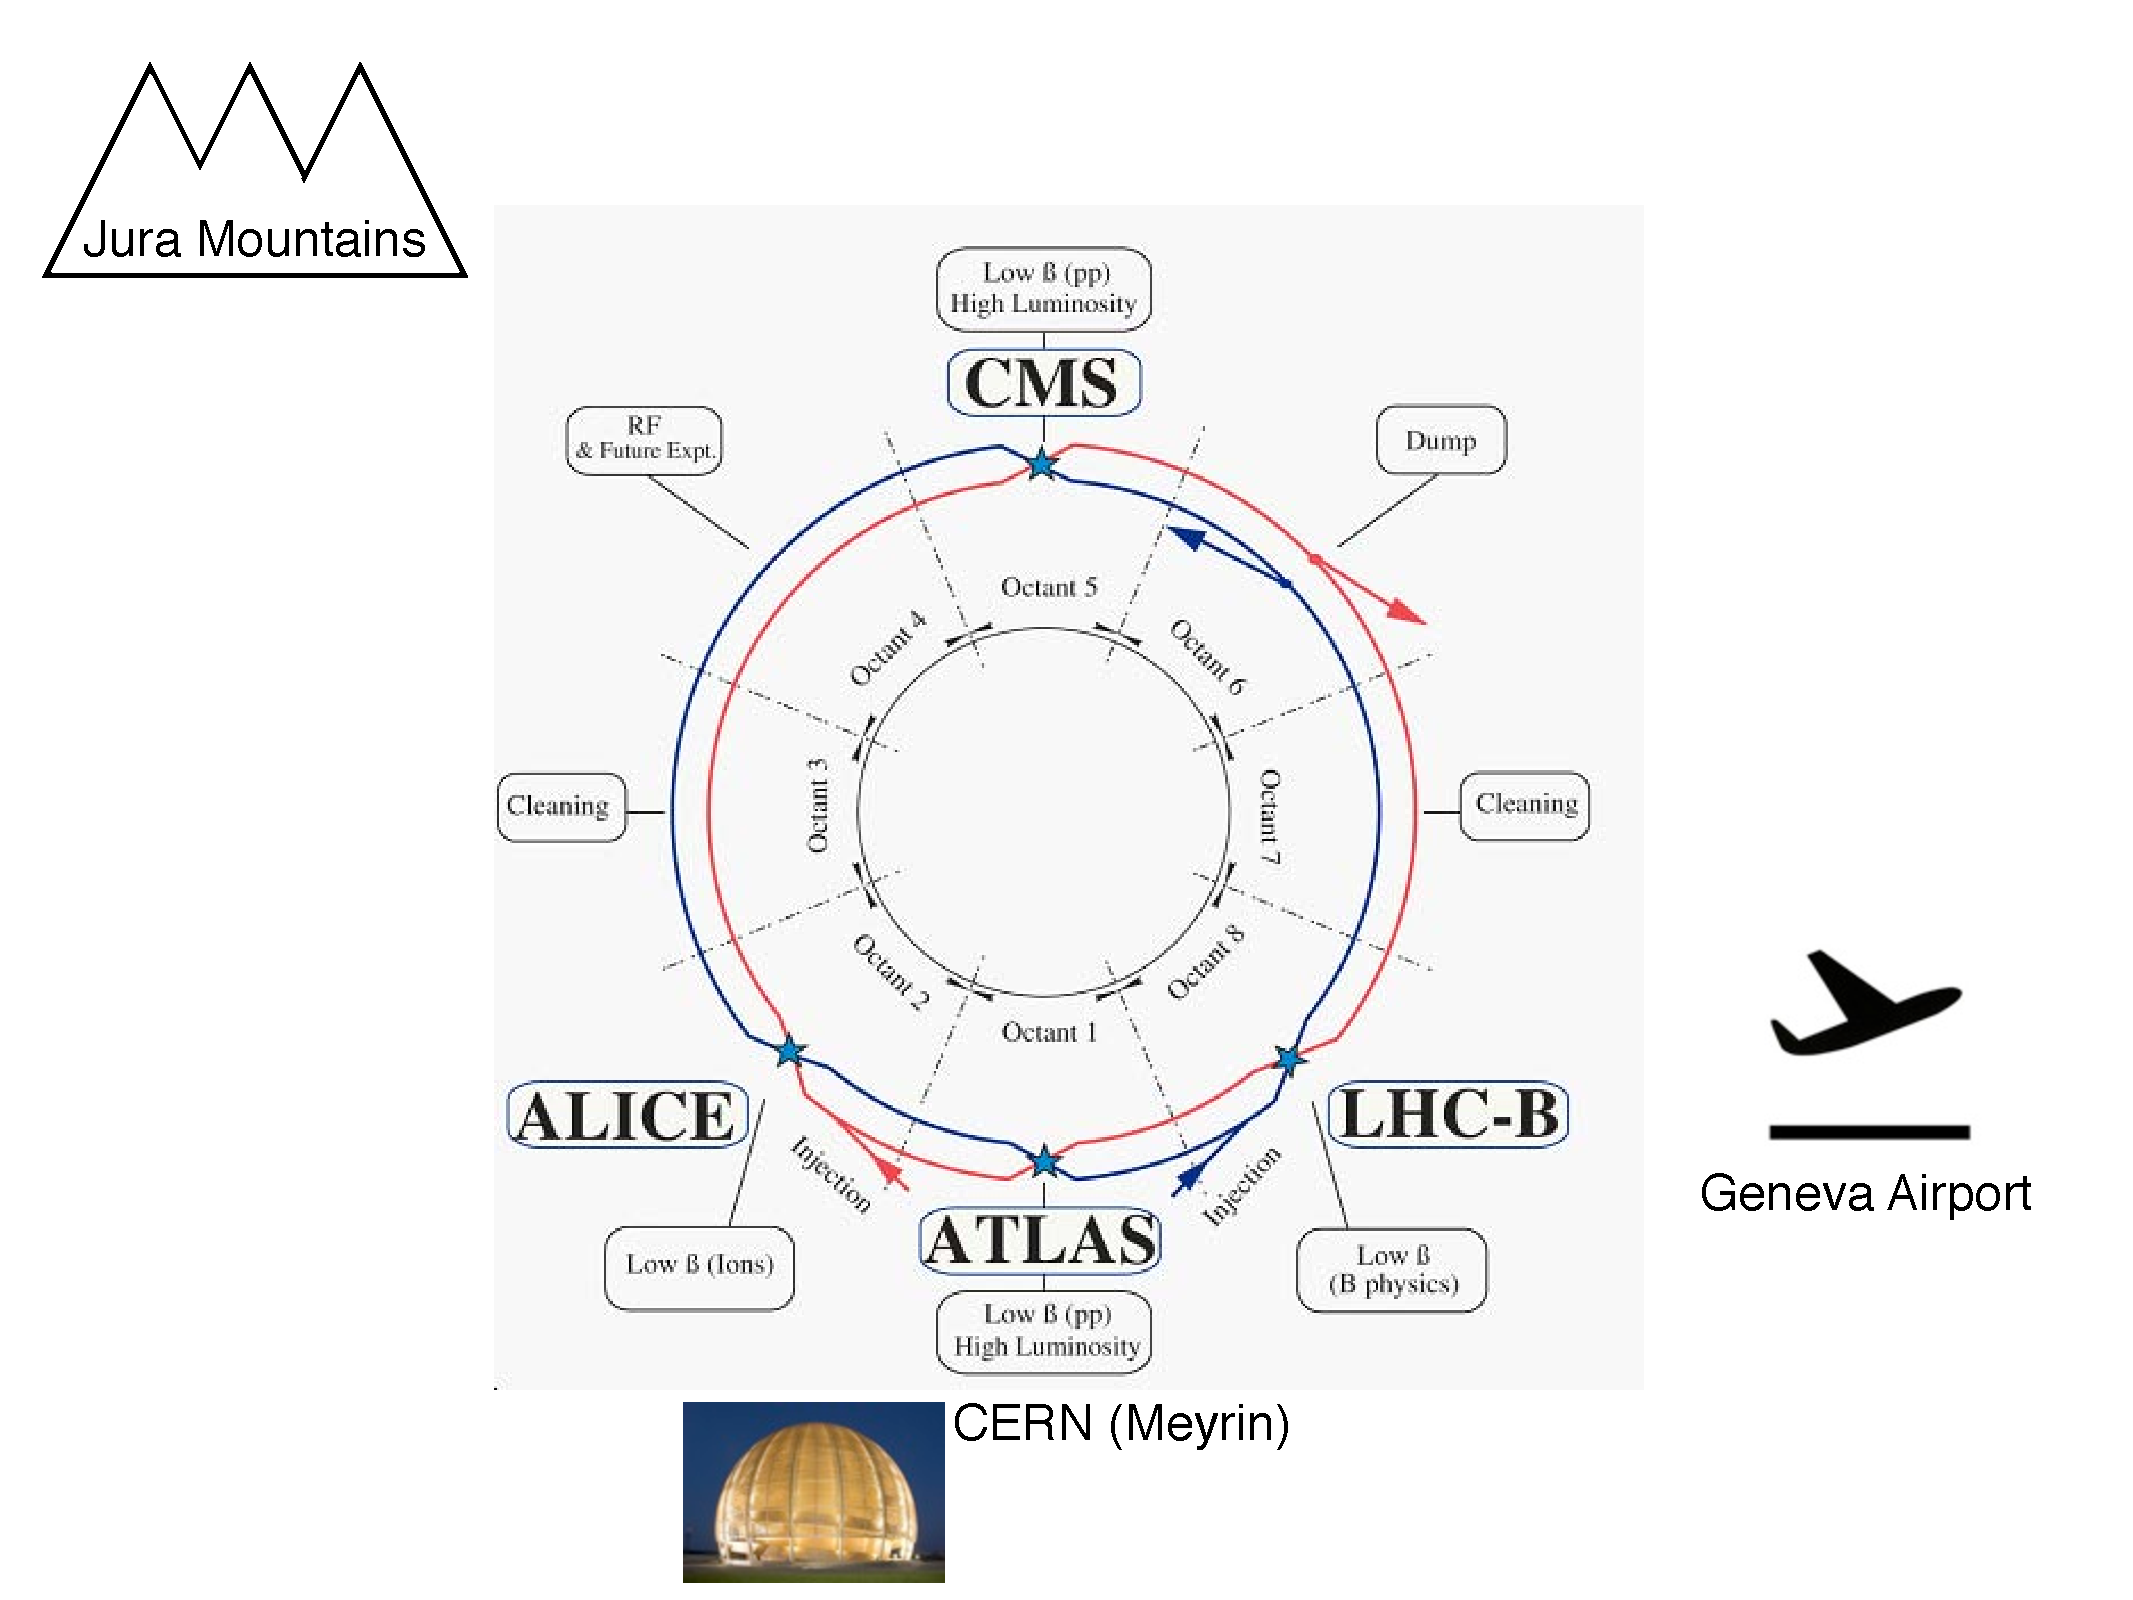
\includegraphics[scale=0.3]{LHC_layout}
	\caption{Bird's-eye view of the LHC ring, showing the locations of the experiments and local landmarks.  Arrows show the beam direction.  The ring figure is reprinted from Fig. 2.1 of ref. \cite{LHC_paper}.  The CERN Globe of Innovation photo comes from ref. \cite{CERN_Globe} and the airplane cartoon comes from ref. \cite{airplane}.}
	\label{fig:LHC_layout}
\end{figure}

To achieve a maximum energy per beam of 7 TeV, the peak magnetic field produced by the dipole magnets must be 8.33 T, demanding the use of superconducting technology.  Due to the like charges of the two beams, two separate magnet systems and evacuated beam pipes must be used to accelerate the protons in opposite directions.  Space limitations in the LHC tunnel, which was previously used for the LEP collider, prevent the installation of two separate rings of magnets, so each dipole instead contains two beam pipe bores and two sets of superconducting coils to produce two fields in opposite directions.  In order to safely operate the magnets at 8.33 T, the cryogenic bath temperature is chosen to be 1.9 K, colder than any other accelerator cryogen and well below the critical temperature of the niobium-titanium (NbTi) superconducting wires of 9.2 K \cite{Flukiger}.  The extremely low bath temperature leads to a lessened heat capacity in the wires and consequently a lower energy threshold for triggering a quench, so movements and heat dissipation within the cables must be controlled more tightly than in previous accelerators.

The LHC beams are arranged in bunches of protons, with each bunch separated by an integer multiple of the 25 ns minimum bunch spacing.  The machine luminosity $L$ is given by

\begin{eqnarray}
L &=& \frac{N_{b}^{2}n_{b}f_{\mathrm{rev}}\gamma_{r}}{4\pi\epsilon_{n}\beta^{*}}F
\end{eqnarray}
%
where $N_{b}$ is the number of protons per bunch (squared for the two beams), $n_{b}$ is the number of bunches per beam, $f_{\mathrm{rev}}$ is the bunch revolution frequency, $\gamma_{r}$ is the relativistic $\gamma$ of the protons, $\epsilon_{n}$ is the normalized transverse beam emittance, $\beta^{*}$ is the value of the $\beta$ function at the collision point, and $F$ is a geometrical factor less than one related to the \textit{crossing angle} of the bunches with respect to the horizontal (ATLAS) or vertical (CMS) planes and the beam size.  The normalized transverse beam emittance is a measure of the RMS spread of the beam in the plane transverse to its direction of motion, irrespective of its energy.  A smaller emittance implies that particles are squeezed into a smaller area in phase space, leading to larger luminosity.  The $\beta$ function is defined as the square of the transverse beam size divided by the emittance.  It describes the oscillations of the transverse beam size as a function of position in the ring.  To achieve high luminosity, $\beta^{*}$ is the minimum of the $\beta$ function, and it is related to the focusing strength of the triplet magnets near the interaction points.  In accelerating sections of the ring, the $\beta$ function gets large so that the proton momenta may be more uniform.  Each piece of the luminosity is limited by safety or design considerations.

Above some saturated bunch intensity, nonlinear beam-beam interactions experienced by the protons during collisions cause the luminosity to scale as $N_{b}$, not $N_{b}^{2}$ \cite{Sun}.  The scale of these interactions is set by $N_{b}/\epsilon_{n}$, and the size of the beam pipe and maximum $\beta$ function limit $\epsilon_{n}$ to 3.75 $\mu\mbox{m}$.  Instabilities are also introduced through interactions between the protons and the wall of the beam pipe that scale with the beam current.  Last but not least, the beam dump and magnet safety systems limit the total stored energy in the ring.  For these reasons, the maximum number of bunches is limited to $1.15\times10^{11}$.  In bunches of this proton multiplicity, the average number of proton-proton collisions per bunch crossing, or \textit{pileup}, in CMS and ATLAS is approximately 20.  This unprecedented level of pileup poses unique triggering, event reconstruction, and analysis challenges for the experiments.

$n_{b}$ can range from zero to 2808 and had a maximum of $\sim1400$ in 2011, corresponding to 50 ns bunch spacing.  $f_{\mathrm{rev}}$ is set by the circumference of the ring to 11.2 kHz \cite{LHC_beam_parameters}.  $\gamma_{r}$ is set by the beam energy, which was 3.5 TeV in 2011.

The mechanical aperture of the triplet assemblies of quadrupole magnets limit the minimum $\beta^{*}$ to $0.55$ \cite{LHC_beam_parameters} and maximum crossing angle to 285 $\mu\mbox{rad}$ \cite{LHC_beam_parameters} at the interaction points.  The purpose of the crossing angle is to prevent parasitic collisions in the 23-m length of shared beam pipe upstream and downstream of the interaction points.

\section{Beam Injection}
\label{sec:Beam Injection}

The ultimate source of protons for the LHC is a bottle of hydrogen connected to the CERN Linac2 linear accelerator, which accelerates the protons up to 50 MeV.  From there they enter the Proton Synchrotron Booster (PSB), which accelerates them to 1.4 GeV, and then the Proton Synchrotron (PS) itself, which brings them to 25 GeV.  The Super Proton Synchrotron (SPS) is the next stage, accelerating the protons to an energy of 450 GeV.  Finally, they leave the SPS and enter the LHC, where they are accelerated to the desired beam energy (3.5 TeV in 2011).  An overview of the LHC injector complex is shown in Figure~\ref{fig:LHC_injector_complex}.

\begin{figure}
	\centering
	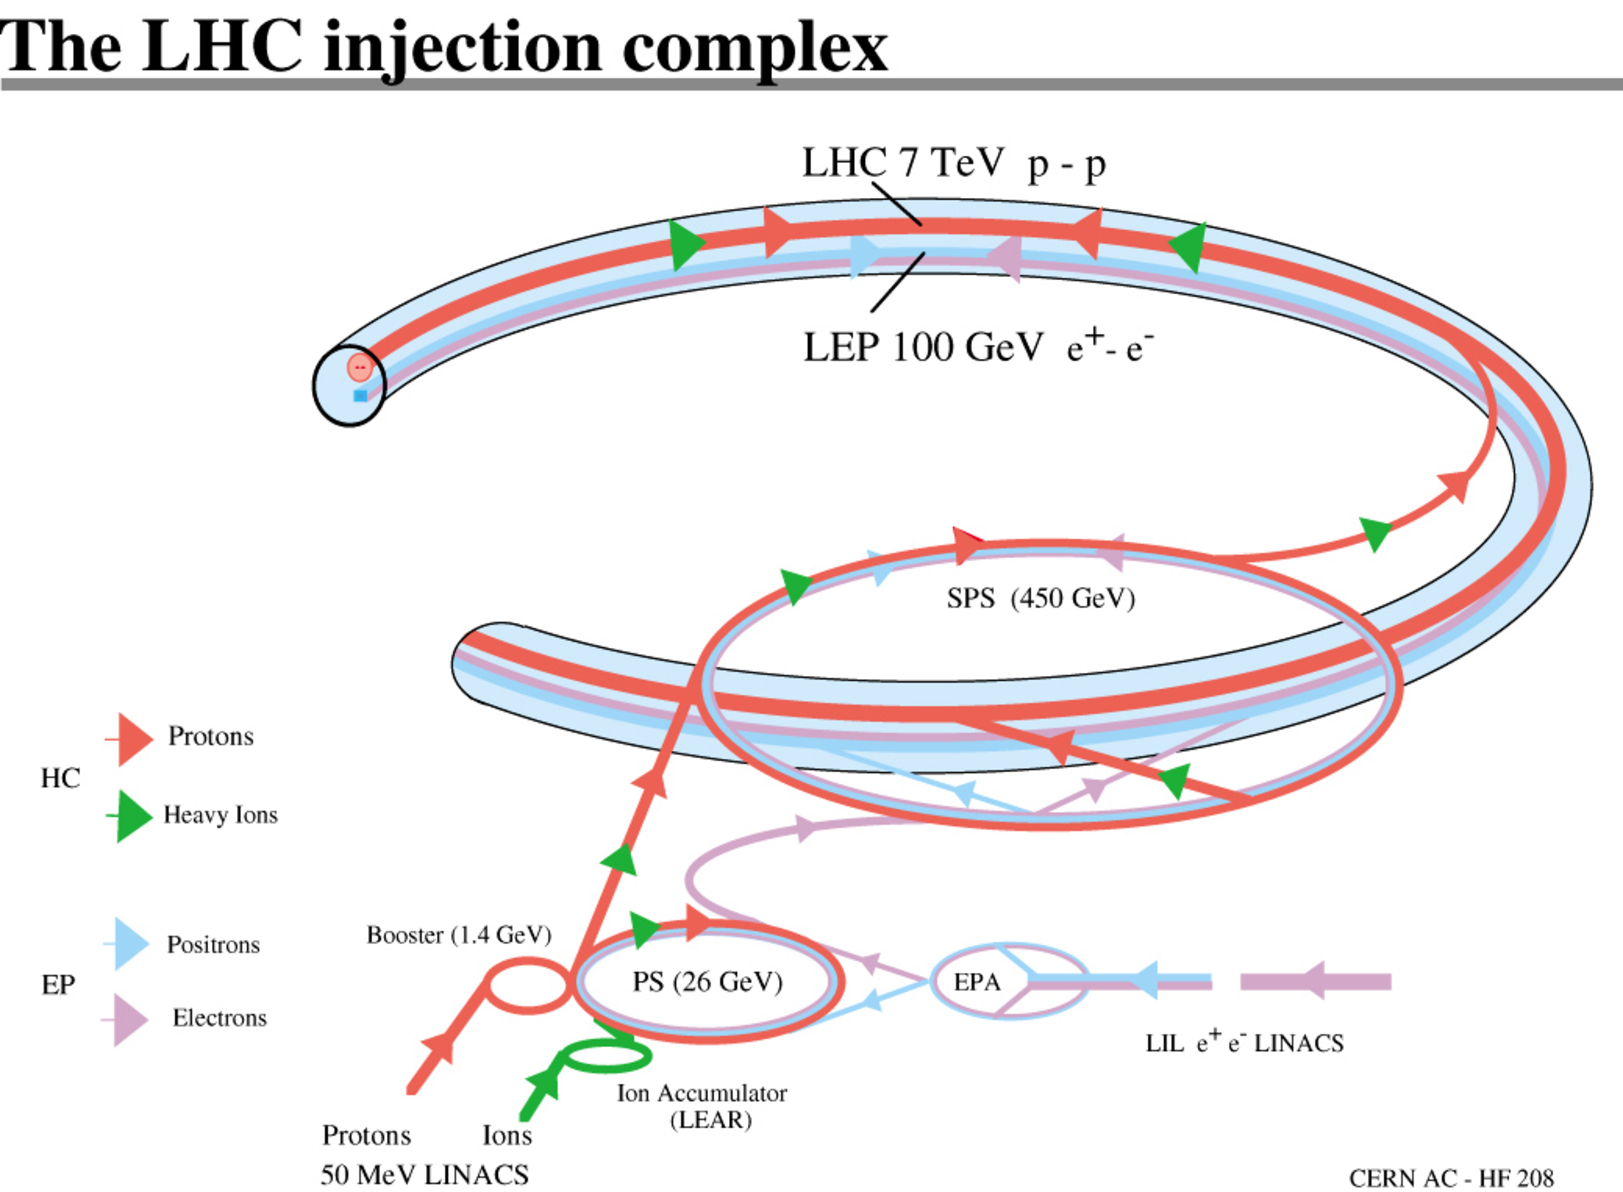
\includegraphics[scale=0.4]{LHC_injector_complex}
	\caption{Overview of the LHC injector complex at CERN \cite{LHC_injector_complex_photo}.}
	\label{fig:LHC_injector_complex}
\end{figure}

The 25-ns spaced bunches (or 50 ns for 2011 operation) are produced in trains of 72 in the PS via a process of splitting six initial bunches into 12 smaller bunches at specified points along the ring.  At the end of each train is a 300 ns (12 bunch) gap, which is an artifact of the splitting process.  The SPS is limited by its maximum allowed bunch intensity to storing three or four PS trains at a time.  There is an 220 ns (8 bunch) gap at the end of each train due to the SPS injection kicker rise time.  The LHC is filled three or four trains at a time from the SPS.  At the end of each three-train and four-train group is a gap of 0.94 $\mu\mbox{s}$ (38 or 39 bunches) due to the LHC injection kicker rise time.  Finally, at the end of an entire 88.924-$\mu\mbox{s}$ long LHC orbit is a gap of 3 $\mu\mbox{s}$ (119 bunches), known as the \textit{abort gap}, to allow for the LHC dump kicker rise time.  The injection scheme is shown in Figure~\ref{fig:LHC_injection_scheme}.

\begin{figure}
	\centering
	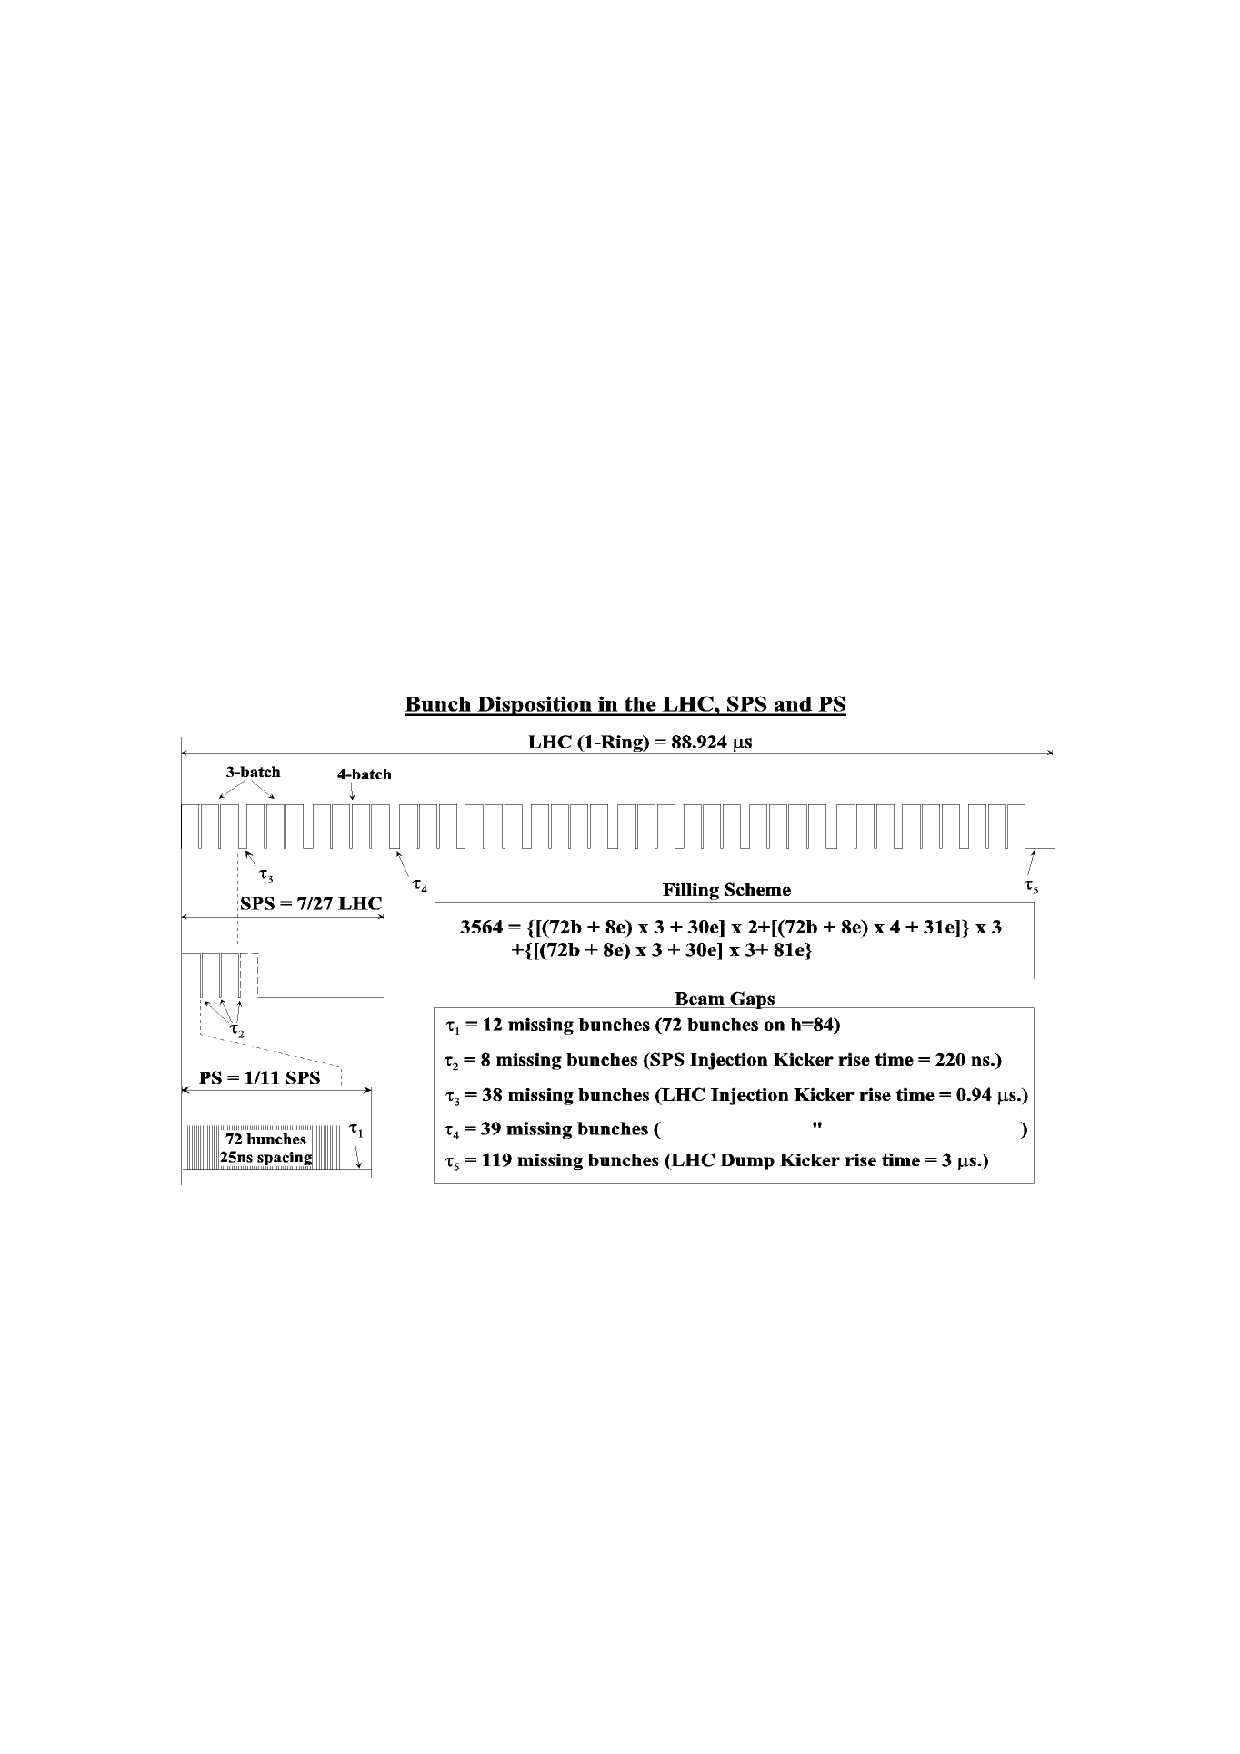
\includegraphics[scale=1.0]{LHC_injection_scheme}
	\caption{LHC injection scheme.  Reprinted from Fig. 12.2 of ref. \cite{LHC_paper}.}
	\label{fig:LHC_injection_scheme}
\end{figure}

LHC injection occurs at points 2 and 8.  At the intersection of the SPS-LHC transfer line and the LHC beam pipe are five septum magnets that deflect the bunches 12 mrad horizontally into orbit.  The septum magnets have a gap into which the beam is injected as well as two separate holes for the circulating beams, as shown in Figure~\ref{fig:LHC_septum_cross_section}.  Four kicker magnets then deflect the bunches 0.85 mrad vertically into orbit.  The kicker magnets supply a pulsed magnetic field with a 0.94 $\mu\mbox{s}$ rise time (see Fig.~\ref{fig:LHC_injection_scheme}) and a 5.84(7.86) $\mu\mbox{s}$ flat top for three-train(four-train) injection (see Figure~\ref{fig:MKI_pulse}).  To limit emittance growth at injection due to over- or under-kicking the injected bunches such that they miss the core of the LHC orbit, the kicker current is limited to $<0.5\%$ flat top ripple in any direction.

\begin{figure}
	\centering
	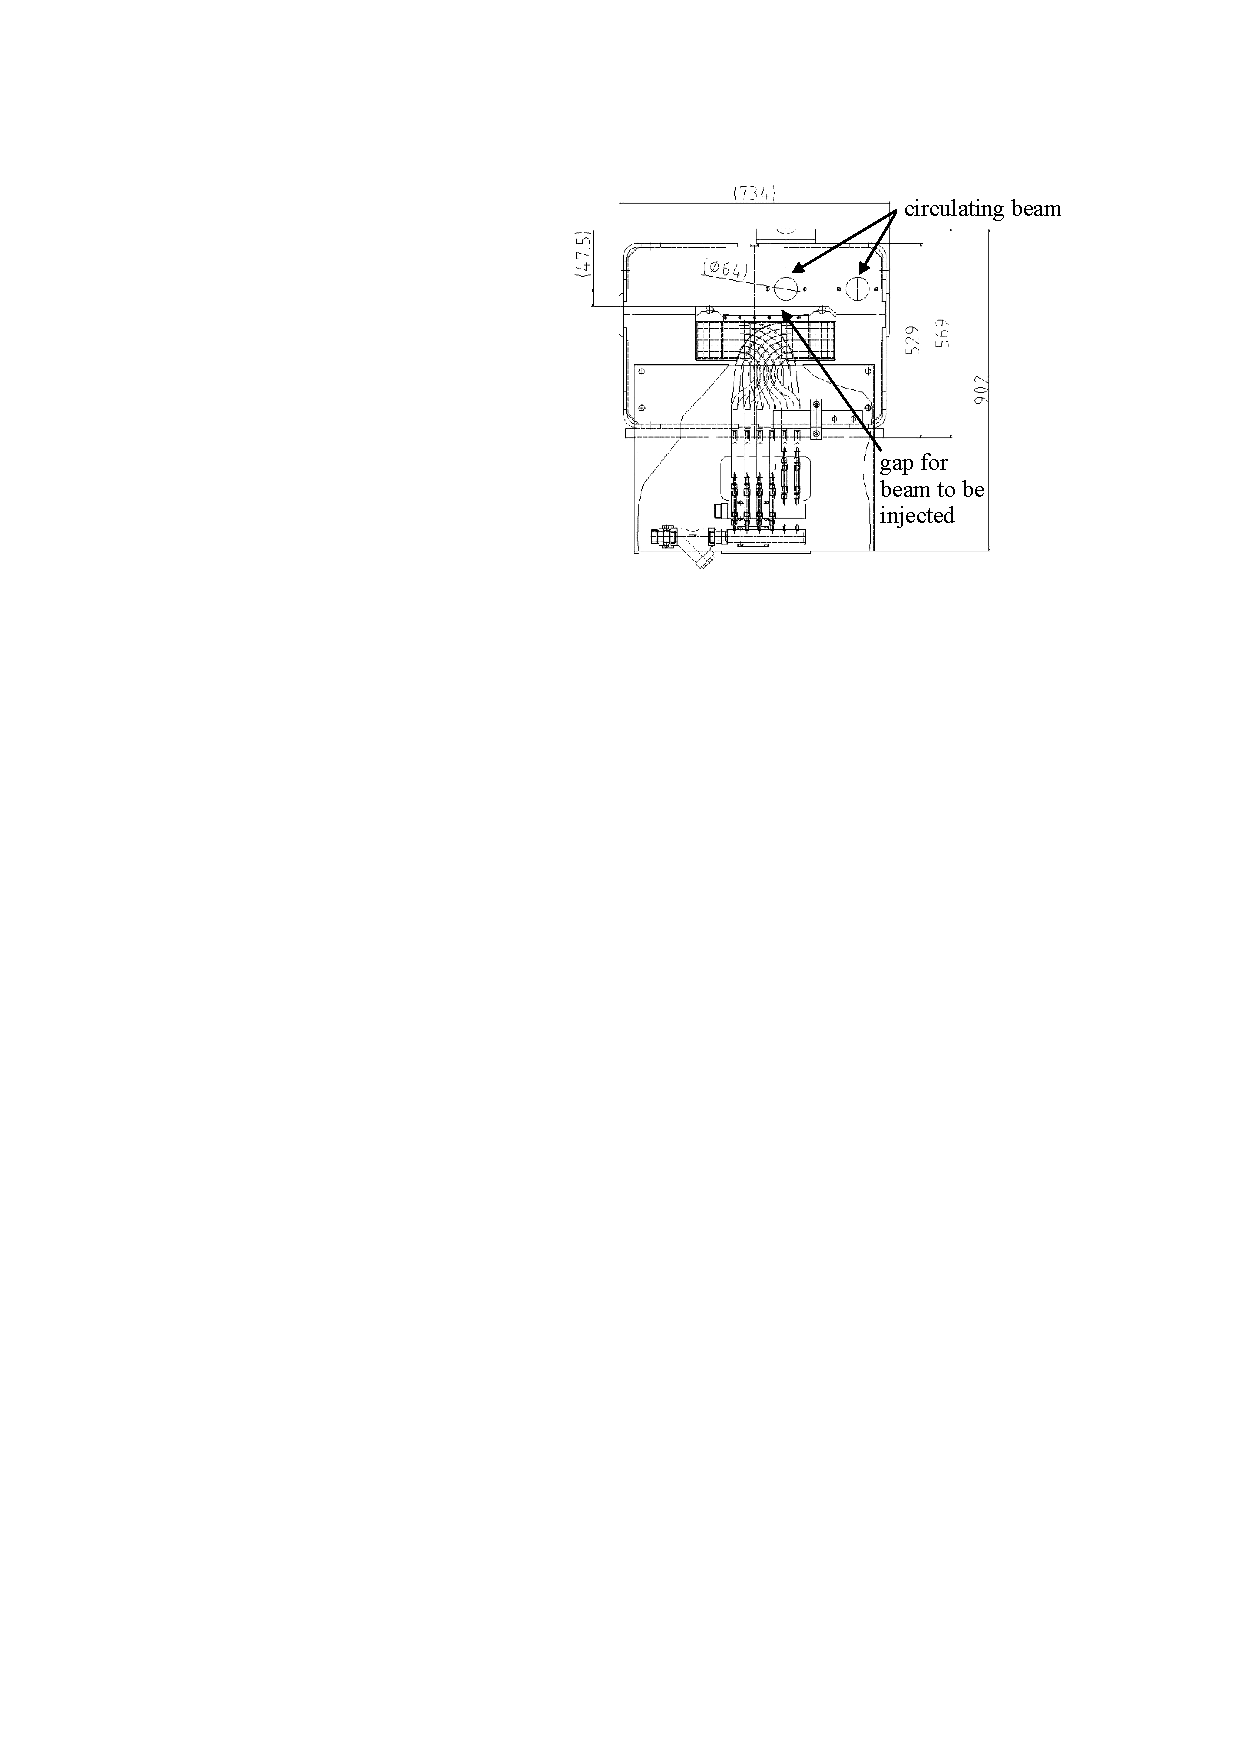
\includegraphics[scale=1.0]{LHC_septum_cross_section}
	\caption{Cross-sectional view of septum magnet (beam direction is into or out of the page) showing the holes for the circulating beams and the separate gap for injected particles.  Reprinted from Fig. 11.2 of ref. \cite{LHC_paper}.}
	\label{fig:LHC_septum_cross_section}
\end{figure}

\begin{figure}
	\centering
	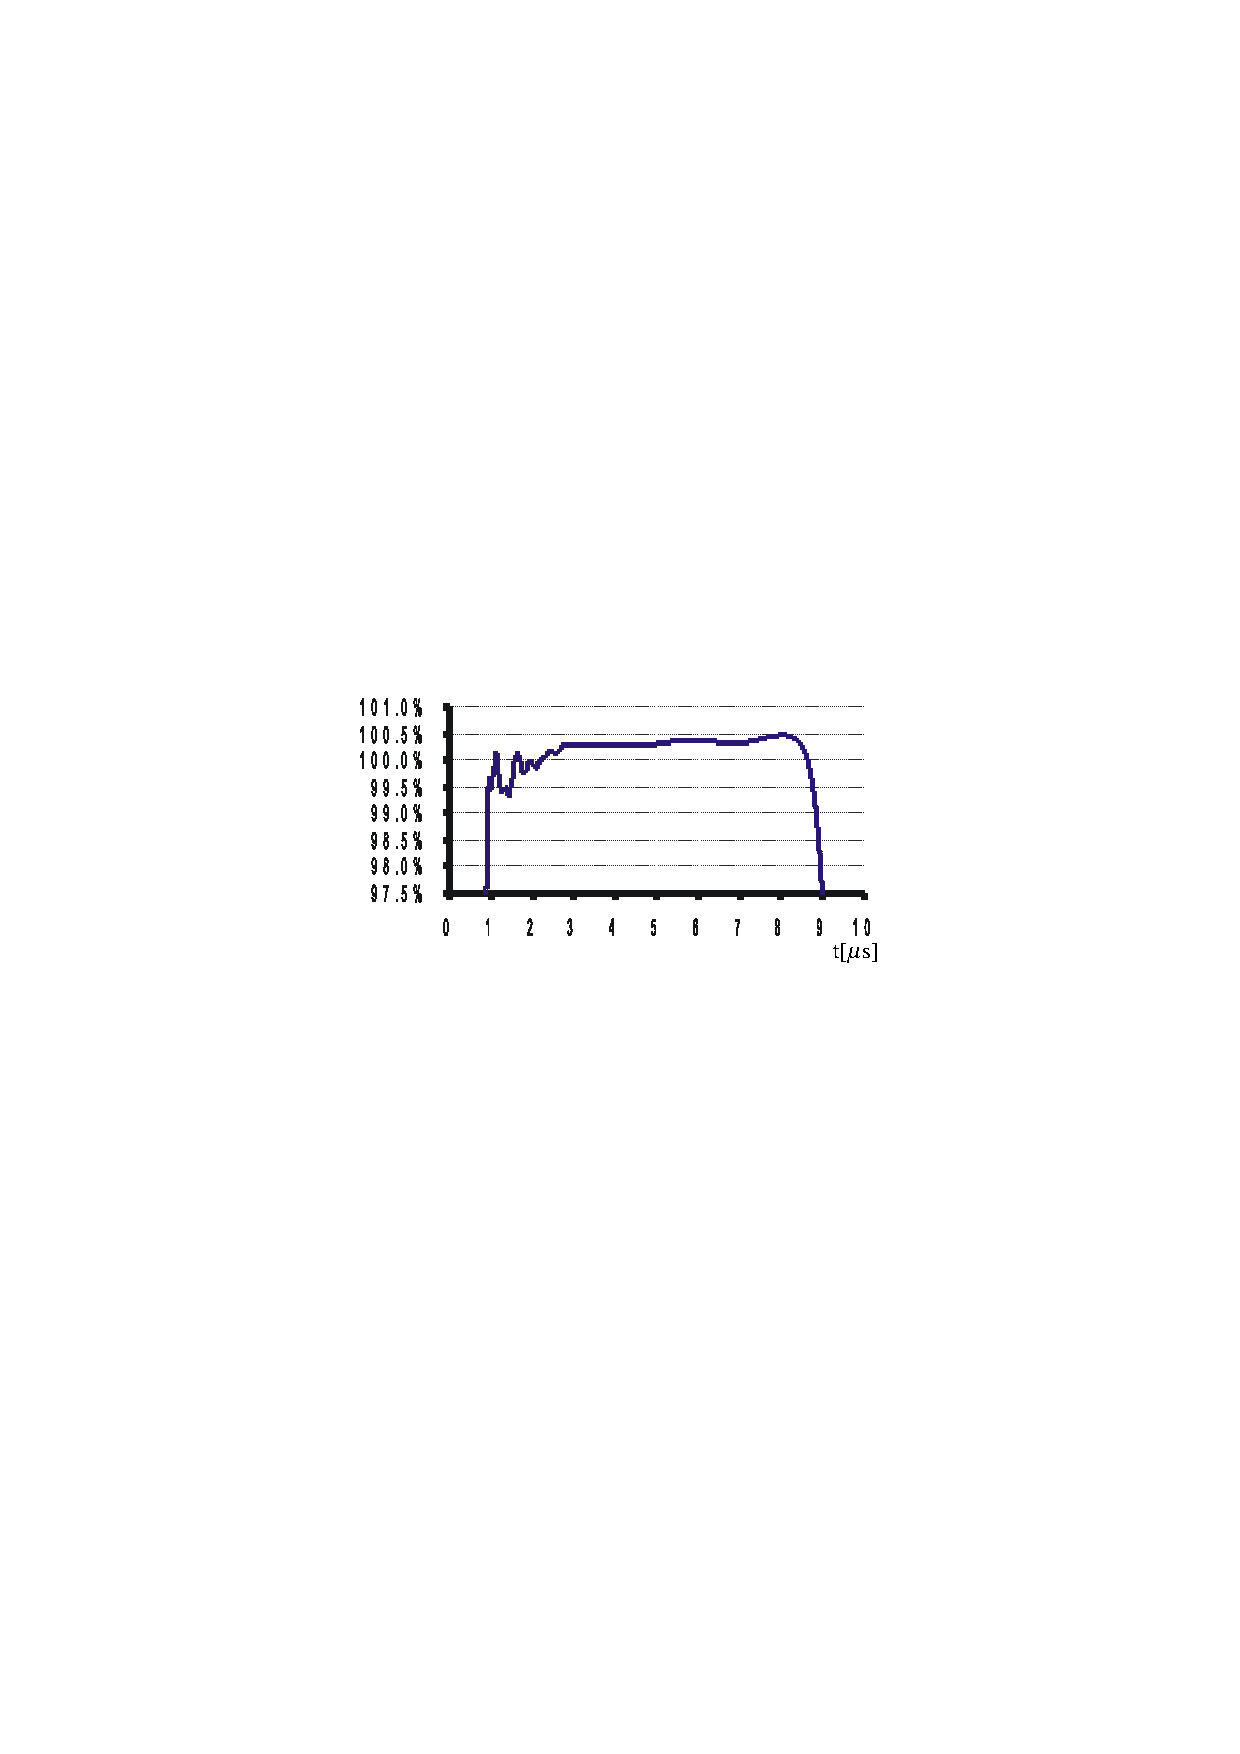
\includegraphics[scale=1.0]{MKI_pulse}
	\caption{LHC injection kicker pulse shape.  The $y$-axis measures percentage of maximum current.  Reprinted from Fig. 11.7 of ref. \cite{LHC_paper}.}
	\label{fig:MKI_pulse}
\end{figure}

\section{Magnets and Cryogenics}
\label{sec:Magnets and Cryogenics}

There are 1232 twin-bore dipole magnets along the LHC ring used for establishing the circular orbit of the protons.  They consist of two evacuated beam pipes, each flanked by its own set of superconducting coils, inside an iron yoke which serves as the 1.9 K cold mass.  The entire assembly sits inside a helium vessel, which is itself surrounded by a vacuum chamber thermally insulating the cold mass from the room temperature LHC cavern.  The entire dipole + cryostat device is $\sim16.5$ m long and weighs about 27.5 t.  A cross-sectional view of the dipole is given in Figure~\ref{fig:LHC_dipole_cross_section}.

\begin{figure}
	\centering
	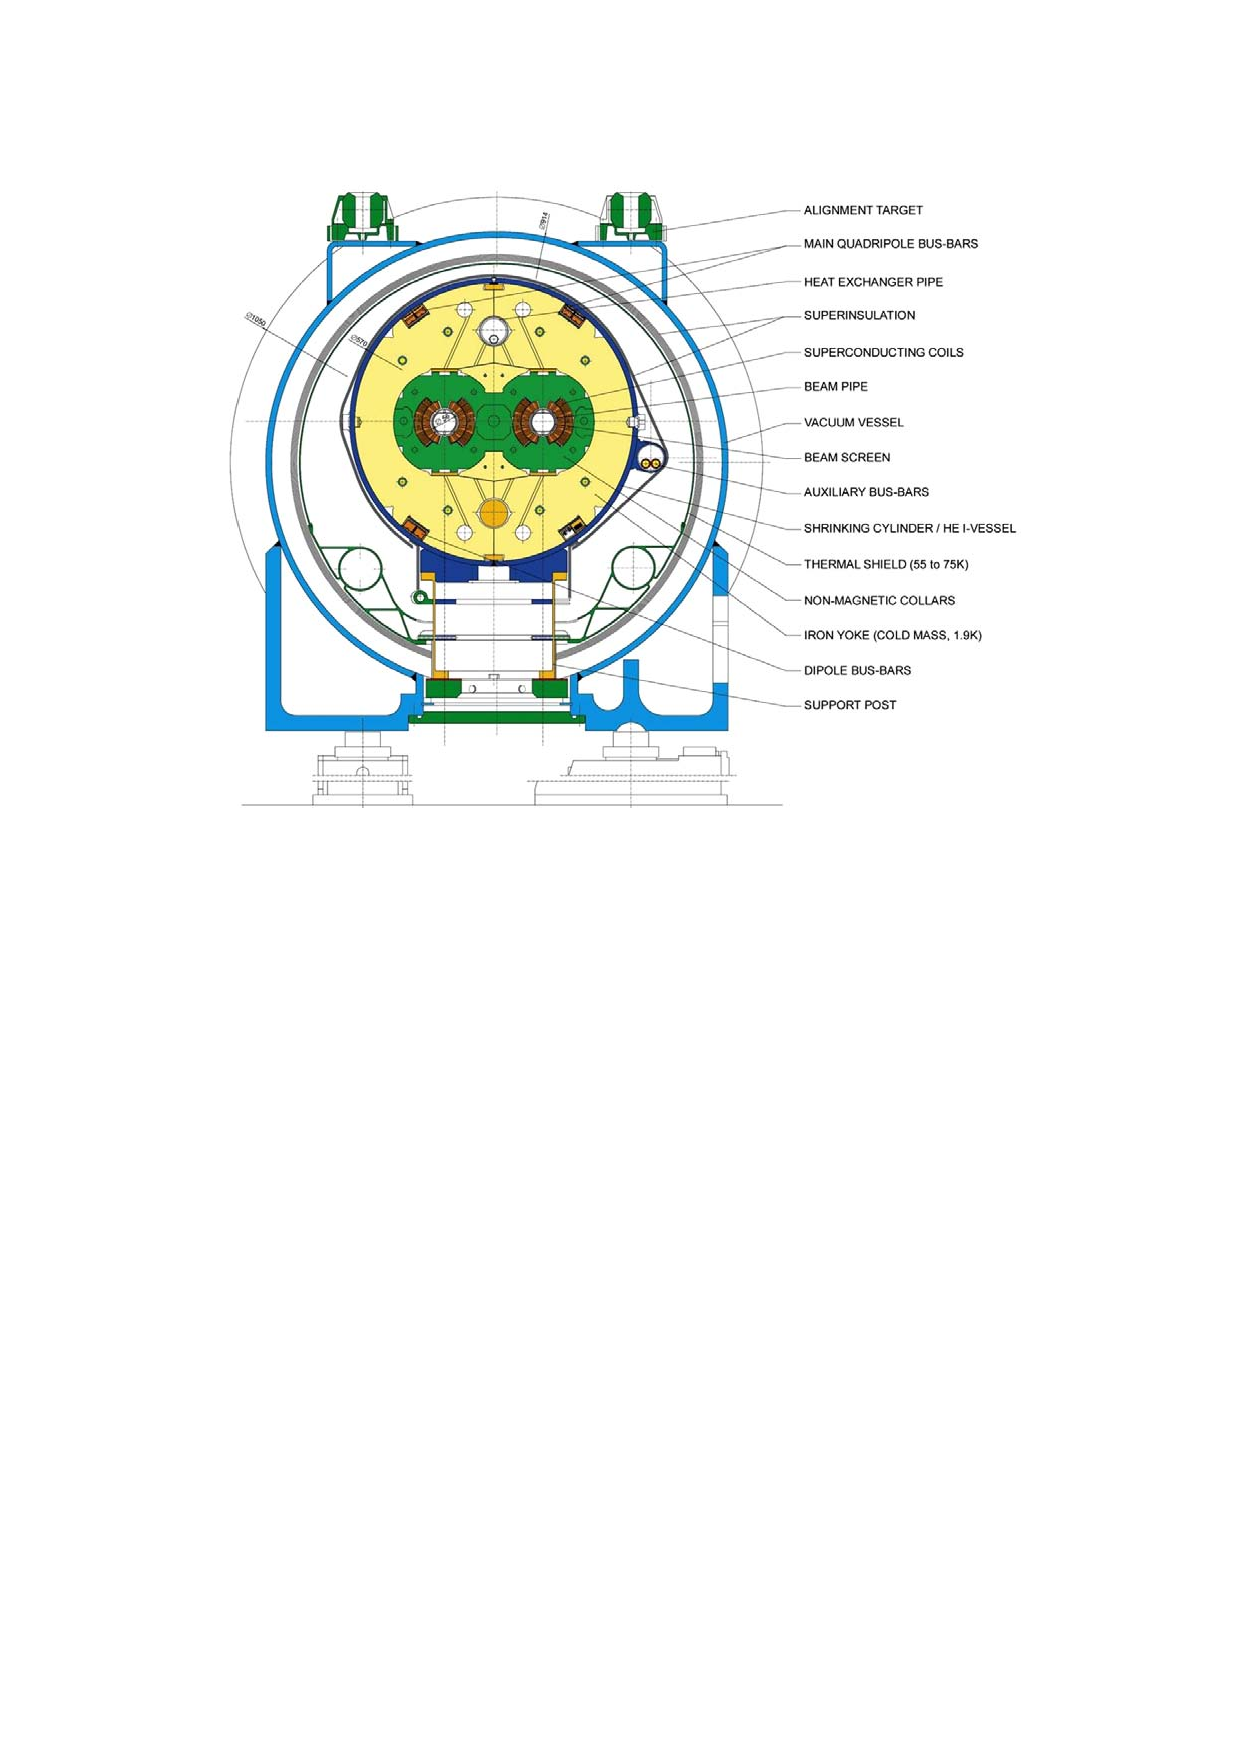
\includegraphics[scale=1.0]{LHC_dipole_cross_section}
	\caption{Cross-sectional view of LHC dipole + cryostat.  Reprinted from Fig. 3.3 of ref. \cite{LHC_paper}.}
	\label{fig:LHC_dipole_cross_section}
\end{figure}

To provide a centripetal Lorentz force on the protons, the dipole field points vertically up or down, depending on the sense of the beam.  The magnetic field lines for a single beam pipe are shown in Figure~\ref{fig:dipole_field}.  Figure~\ref{fig:coil_windings} shows the coil windings in two bores.  To provide the correct field direction, the coils are wound around blocks that are $\sim14$ m long (the length of the dipole), so that each winding has a circumference of $\sim28$ m.

\begin{figure}
	\centering
	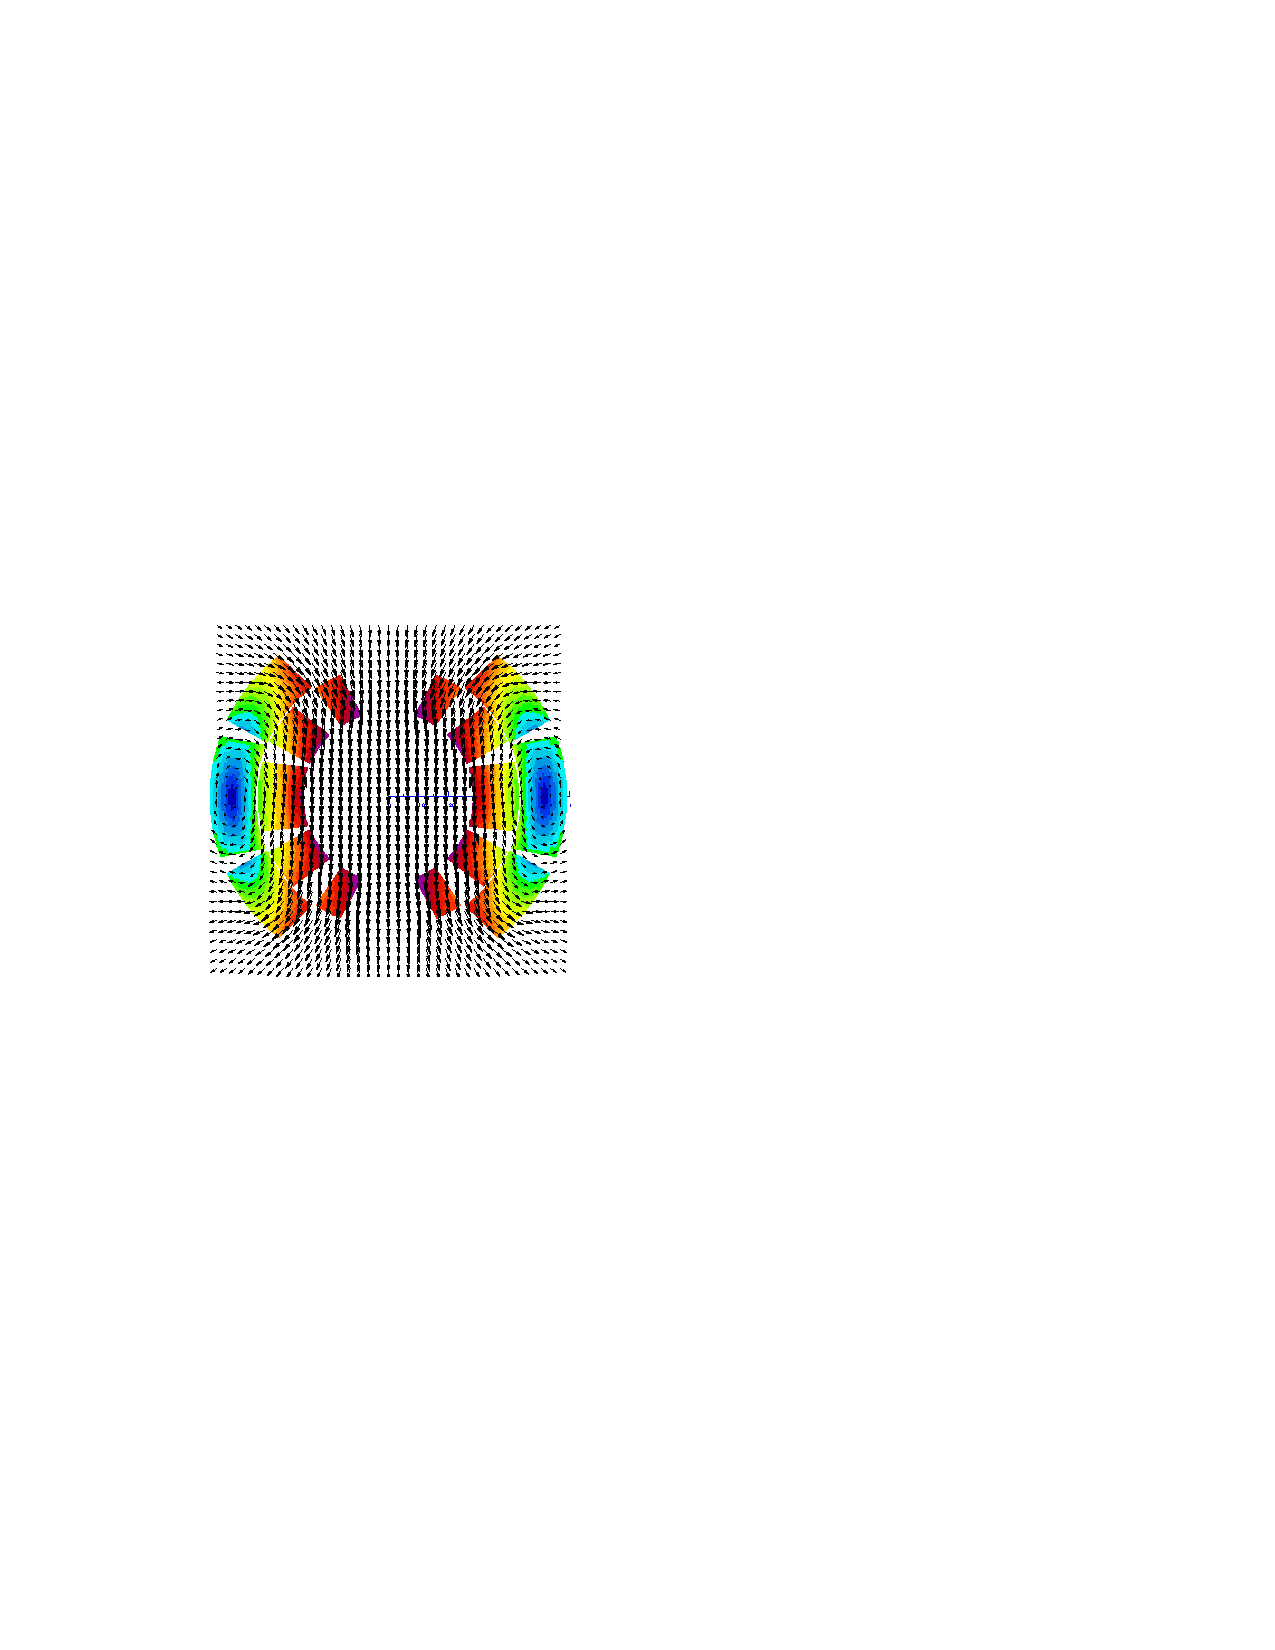
\includegraphics[scale=1.0]{dipole_field}
	\caption{Magnetic field lines of the dipole field.  The beam direction is into the page.  Reprinted from Fig. 4 of ref. \cite{Komorowski}.}
	\label{fig:dipole_field}
\end{figure}

\begin{figure}
	\centering
	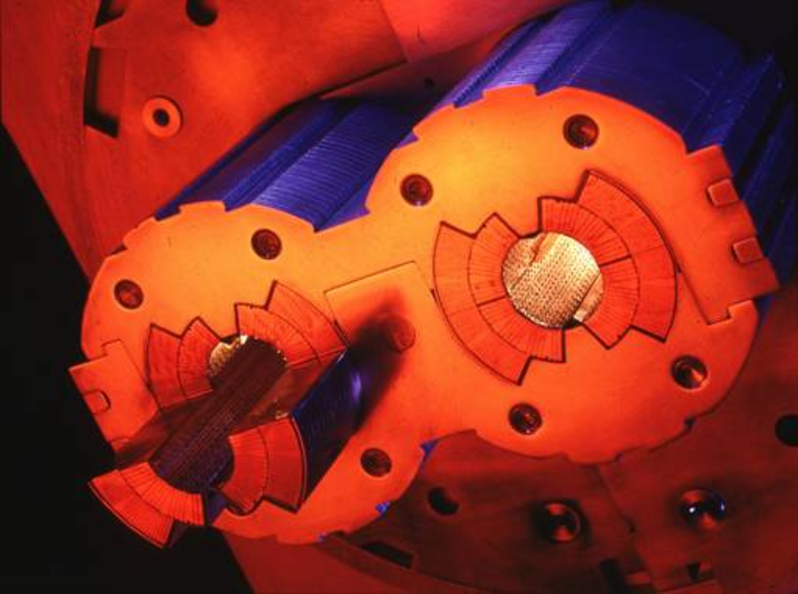
\includegraphics[scale=1.0]{coil_windings}
	\caption{Superconducting coils in a twin-bore dipole \cite{LHC_outreach_magnets}.}
	\label{fig:coil_windings}
\end{figure}

In addition to the dipoles, a number of different types of orbit corrector magnets are installed throughout the ring.  The main quadrupole magnets, as well as higher order field corrector magnets, are located in the arcs and short straight sections.  The function of these magnets is to provide fine grained control over the magnetic field in order to keep the bunches in the proper orbit and control the emittance and $\beta$ functions.

In the straight sections, there are four specialized types of magnets related to SPS extraction and bringing the beams into collision.  Matching section quadrupoles near the transfer lines help to match the injected bunch orbit to the circulating bunch orbit.  Dispersion suppressors, consisting of dipoles and quadrupoles, help to reduce beam dispersion near the collision points due to off-momentum protons.  Matching section separation dipoles control the separation between the two beams near the collision points.  The magnets that perform the final squeeze of the beams before collision, called the low-$\beta$ inner triplets, must provide a very high field gradient of 215 T/m, withstand a high radiation dose, and sustain high heat loads in the superconducting coils.

The superfluid helium cryogen is delivered to the magnets via a distribution line from the main refrigerator.  A cross section of the LHC tunnel, showing the cryogen delivery apparatus for a dipole, is shown in Figure~\ref{fig:tunnel_cross_section}.

\begin{figure}
	\centering
	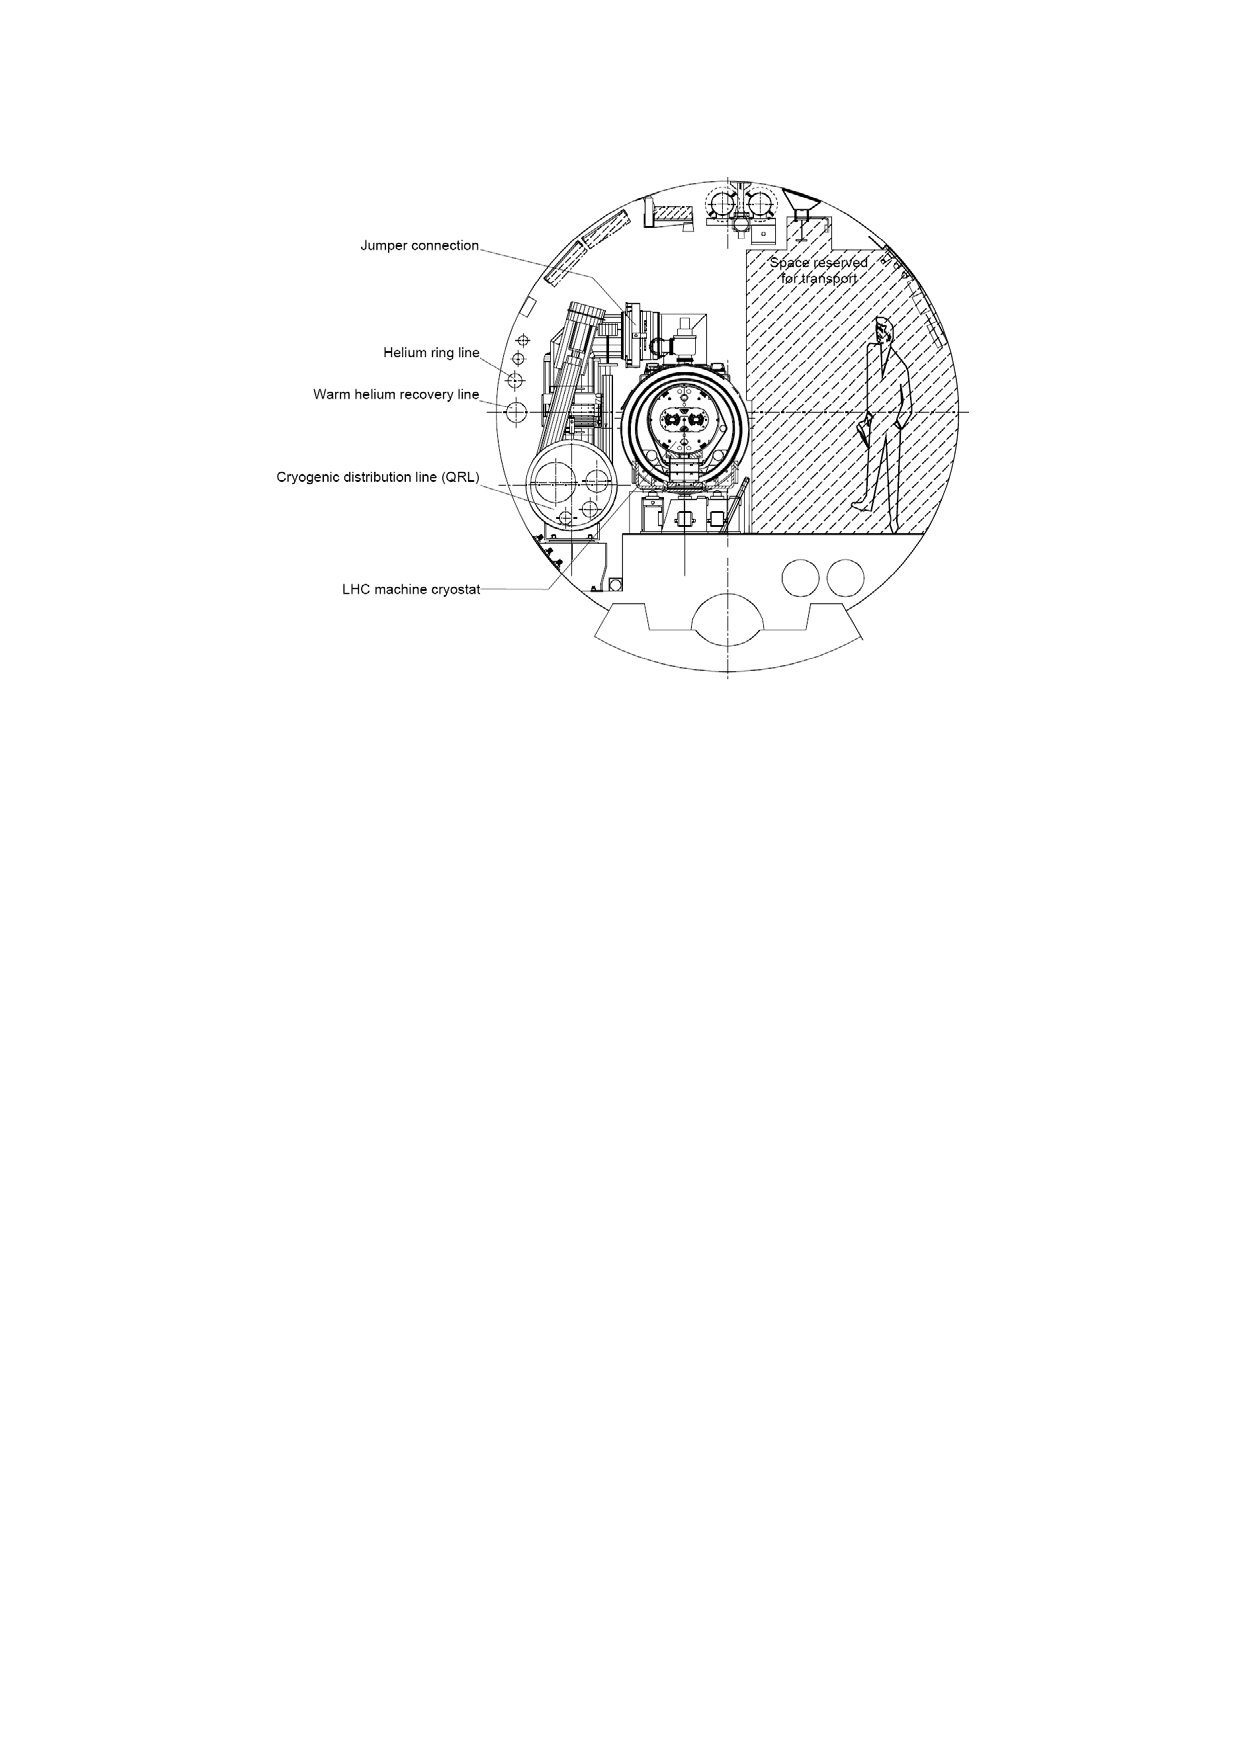
\includegraphics[scale=1.0]{tunnel_cross_section}
	\caption{Cross section of the LHC tunnel, showing the cryogen delivery apparatus for a dipole.  Reprinted from Fig. 7.1 of ref. \cite{LHC_paper}.}
	\label{fig:tunnel_cross_section}
\end{figure}

\section{Radiofrequency Cavities}
\label{sec:Radiofrequency Cavities}

LHC bunches are captured and accelerated in 400 MHz superconducting radiofrequency (RF) cavities.  400 MHz defines the bunch length of $\lesssim2$ ns.  As bunches pass through the cavities, the oscillating electric field is at its peak and accelerates the protons through a potential difference of 2 MV per cavity (16 MV per turn).  The finite bunch length is due to particles that arrive out of phase with the electric field due to deviations in their momenta from the nominal.  During a ramp of the beam energy from 450 GeV to 3.5 or 7 TeV, bunches repeatedly travel around the ring, receiving an energy kick each time, until the desired energy is reached.  Feedback from the RF accelerating system causes an increase in magnet current to keep the bunches in a fixed orbit.

Superconducting material (niobium) coats the cylindrical walls of the cavity.  RF power is coupled to the cavity via a klystron.  The RF electric field standing wave is set up across the cavity in the beam direction.  The transverse magnetic field dissipates some energy into the walls, but much less than in a normal conducting cavity.

\end{document}